% Options for packages loaded elsewhere
\PassOptionsToPackage{unicode}{hyperref}
\PassOptionsToPackage{hyphens}{url}
%
\documentclass[
]{article}
\usepackage{amsmath,amssymb}
\usepackage{lmodern}
\usepackage{ifxetex,ifluatex}
\ifnum 0\ifxetex 1\fi\ifluatex 1\fi=0 % if pdftex
  \usepackage[T1]{fontenc}
  \usepackage[utf8]{inputenc}
  \usepackage{textcomp} % provide euro and other symbols
\else % if luatex or xetex
  \usepackage{unicode-math}
  \defaultfontfeatures{Scale=MatchLowercase}
  \defaultfontfeatures[\rmfamily]{Ligatures=TeX,Scale=1}
\fi
% Use upquote if available, for straight quotes in verbatim environments
\IfFileExists{upquote.sty}{\usepackage{upquote}}{}
\IfFileExists{microtype.sty}{% use microtype if available
  \usepackage[]{microtype}
  \UseMicrotypeSet[protrusion]{basicmath} % disable protrusion for tt fonts
}{}
\makeatletter
\@ifundefined{KOMAClassName}{% if non-KOMA class
  \IfFileExists{parskip.sty}{%
    \usepackage{parskip}
  }{% else
    \setlength{\parindent}{0pt}
    \setlength{\parskip}{6pt plus 2pt minus 1pt}}
}{% if KOMA class
  \KOMAoptions{parskip=half}}
\makeatother
\usepackage{xcolor}
\IfFileExists{xurl.sty}{\usepackage{xurl}}{} % add URL line breaks if available
\IfFileExists{bookmark.sty}{\usepackage{bookmark}}{\usepackage{hyperref}}
\hypersetup{
  pdftitle={CLASE 110-DATOS ORDINALES},
  pdfauthor={VICTOR MIGUEL TERRON MACIAS},
  hidelinks,
  pdfcreator={LaTeX via pandoc}}
\urlstyle{same} % disable monospaced font for URLs
\usepackage[margin=1in]{geometry}
\usepackage{color}
\usepackage{fancyvrb}
\newcommand{\VerbBar}{|}
\newcommand{\VERB}{\Verb[commandchars=\\\{\}]}
\DefineVerbatimEnvironment{Highlighting}{Verbatim}{commandchars=\\\{\}}
% Add ',fontsize=\small' for more characters per line
\usepackage{framed}
\definecolor{shadecolor}{RGB}{248,248,248}
\newenvironment{Shaded}{\begin{snugshade}}{\end{snugshade}}
\newcommand{\AlertTok}[1]{\textcolor[rgb]{0.94,0.16,0.16}{#1}}
\newcommand{\AnnotationTok}[1]{\textcolor[rgb]{0.56,0.35,0.01}{\textbf{\textit{#1}}}}
\newcommand{\AttributeTok}[1]{\textcolor[rgb]{0.77,0.63,0.00}{#1}}
\newcommand{\BaseNTok}[1]{\textcolor[rgb]{0.00,0.00,0.81}{#1}}
\newcommand{\BuiltInTok}[1]{#1}
\newcommand{\CharTok}[1]{\textcolor[rgb]{0.31,0.60,0.02}{#1}}
\newcommand{\CommentTok}[1]{\textcolor[rgb]{0.56,0.35,0.01}{\textit{#1}}}
\newcommand{\CommentVarTok}[1]{\textcolor[rgb]{0.56,0.35,0.01}{\textbf{\textit{#1}}}}
\newcommand{\ConstantTok}[1]{\textcolor[rgb]{0.00,0.00,0.00}{#1}}
\newcommand{\ControlFlowTok}[1]{\textcolor[rgb]{0.13,0.29,0.53}{\textbf{#1}}}
\newcommand{\DataTypeTok}[1]{\textcolor[rgb]{0.13,0.29,0.53}{#1}}
\newcommand{\DecValTok}[1]{\textcolor[rgb]{0.00,0.00,0.81}{#1}}
\newcommand{\DocumentationTok}[1]{\textcolor[rgb]{0.56,0.35,0.01}{\textbf{\textit{#1}}}}
\newcommand{\ErrorTok}[1]{\textcolor[rgb]{0.64,0.00,0.00}{\textbf{#1}}}
\newcommand{\ExtensionTok}[1]{#1}
\newcommand{\FloatTok}[1]{\textcolor[rgb]{0.00,0.00,0.81}{#1}}
\newcommand{\FunctionTok}[1]{\textcolor[rgb]{0.00,0.00,0.00}{#1}}
\newcommand{\ImportTok}[1]{#1}
\newcommand{\InformationTok}[1]{\textcolor[rgb]{0.56,0.35,0.01}{\textbf{\textit{#1}}}}
\newcommand{\KeywordTok}[1]{\textcolor[rgb]{0.13,0.29,0.53}{\textbf{#1}}}
\newcommand{\NormalTok}[1]{#1}
\newcommand{\OperatorTok}[1]{\textcolor[rgb]{0.81,0.36,0.00}{\textbf{#1}}}
\newcommand{\OtherTok}[1]{\textcolor[rgb]{0.56,0.35,0.01}{#1}}
\newcommand{\PreprocessorTok}[1]{\textcolor[rgb]{0.56,0.35,0.01}{\textit{#1}}}
\newcommand{\RegionMarkerTok}[1]{#1}
\newcommand{\SpecialCharTok}[1]{\textcolor[rgb]{0.00,0.00,0.00}{#1}}
\newcommand{\SpecialStringTok}[1]{\textcolor[rgb]{0.31,0.60,0.02}{#1}}
\newcommand{\StringTok}[1]{\textcolor[rgb]{0.31,0.60,0.02}{#1}}
\newcommand{\VariableTok}[1]{\textcolor[rgb]{0.00,0.00,0.00}{#1}}
\newcommand{\VerbatimStringTok}[1]{\textcolor[rgb]{0.31,0.60,0.02}{#1}}
\newcommand{\WarningTok}[1]{\textcolor[rgb]{0.56,0.35,0.01}{\textbf{\textit{#1}}}}
\usepackage{graphicx}
\makeatletter
\def\maxwidth{\ifdim\Gin@nat@width>\linewidth\linewidth\else\Gin@nat@width\fi}
\def\maxheight{\ifdim\Gin@nat@height>\textheight\textheight\else\Gin@nat@height\fi}
\makeatother
% Scale images if necessary, so that they will not overflow the page
% margins by default, and it is still possible to overwrite the defaults
% using explicit options in \includegraphics[width, height, ...]{}
\setkeys{Gin}{width=\maxwidth,height=\maxheight,keepaspectratio}
% Set default figure placement to htbp
\makeatletter
\def\fps@figure{htbp}
\makeatother
\setlength{\emergencystretch}{3em} % prevent overfull lines
\providecommand{\tightlist}{%
  \setlength{\itemsep}{0pt}\setlength{\parskip}{0pt}}
\setcounter{secnumdepth}{-\maxdimen} % remove section numbering
\ifluatex
  \usepackage{selnolig}  % disable illegal ligatures
\fi

\title{CLASE 110-DATOS ORDINALES}
\author{VICTOR MIGUEL TERRON MACIAS}
\date{14/6/2021}

\begin{document}
\maketitle

\hypertarget{datos-ordinales}{%
\section{DATOS ORDINALES}\label{datos-ordinales}}

Recordad que la \textbf{diferencia} entre un \textbf{dato ordinal} y un
\textbf{dato cualitativo} es que el ordinal que vamos a trabajar aquí
sigue describiendo una cualidad de un objeto o una cualidad de un
individuo. Pero ahora el dato cualitativo presenta unas características
que expresan datos ordinales es decir que presentan un orden natural que
permite ir acumulando observaciones es decir podremos contar para cada
nivel cuántas observaciones hay por debajo de ese nivel ya no sólo
podemos contar observaciones frecuencias absolutas las llamábamos de
cada uno de los niveles sino frecuencias menores o iguales que las de un
nivel dado.

Un caso frecuente van a ser las escalas Flicker que se utilizan para
conocer la opinión de un grupo de personas sobre un tema o un tema
determinado por ejemplo si vamos a la Wikipedia y buscamos las escalas y
qué vais a ver que la misma Wikipedia aparece pues las típicas encuestas
que conoceis y que seguramente alguna vez os han llevado a cabo o son
las encuestas de cinco puntos respecto a una afirmación cuando te gusta
ir al cine estás totalmente desacuerdo en desacuerdo ni de acuerdo ni
desacuerdo de acuerdo o totalmente de acuerdo.

Normalmente las escalas de Ticker presentan unas respuestas de este
estilo donde podréis ver que la respuesta es una categoría Manen sigue
siendo una categoría como lo era anteriormente pero con la diferencia de
que estas categorías ahora tienen cierto orden y que responder uno en la
pregunta Te gusta ir al cine es estar menos en estar más en desacuerdo
que responder cuatro que significa estar de acuerdo que te gusta ir al
cine de acuerdo por tanto esa va a ser la diferencia grande que nos va a
permitir diferenciar entre un dato ordinal y un dato cualitativo veréis
que en erre pues es una pequeña variante de lo que ya conocéis y que
habiendo trabajado tanto el tema de las cualidades o los datos
cualitativos no va a costar demasiado emigrar ahora a los datos
ordinales.

\hypertarget{frecuencais-acumuladas-en-datos-ordinales}{%
\section{FRECUENCAIS ACUMULADAS EN DATOS
ORDINALES}\label{frecuencais-acumuladas-en-datos-ordinales}}

Los datos ordinales son parecidos a los cualitativos, en el sentido de
que son cualidades de los individuos u objetos.

La diferencia existente entre los datos cualitativos y los ordinales
reside en las características que expresan. En el caso de los ordinales,
éstas tienen un orden natural que permite acumular observaciones.

Escalas likert son 1. Totalmente de acuerdo 2. En desacuerdo 3. Ni
deacuerdo ni en desacuerdo 4. Desacuerdo 5. Totalmente en desacuerdo

\hypertarget{frecuencia-acumulada-en-datos-ordinales}{%
\subsection{FRECUENCIA ACUMULADA EN DATOS
ORDINALES}\label{frecuencia-acumulada-en-datos-ordinales}}

\textbf{Ejemplo1}

Suponed que tenemos una muestra de 15 estudiantes de los cuales sabemos
su nota en examen de estadística. Clasificamos todos estos resultados en
suspenso, aprobado, notable y excelente, las notas han sido las
siguientes:

S,A,N,Ex,S,S,Ex,Ex,N,A,A,A,A,A,N,S

Para calculo de frecuencia absoluta se usa la funcion \textbf{table()}

Para crear un array de datos ordinales se utiliza la funcion
\textbf{ordered(c())}

\begin{Shaded}
\begin{Highlighting}[]
\NormalTok{notas}\OtherTok{=}\FunctionTok{ordered}\NormalTok{(}\FunctionTok{c}\NormalTok{(}\StringTok{"S"}\NormalTok{,}\StringTok{"A"}\NormalTok{,}\StringTok{"N"}\NormalTok{,}\StringTok{"Ex"}\NormalTok{,}\StringTok{"S"}\NormalTok{,}\StringTok{"S"}\NormalTok{,}\StringTok{"Ex"}\NormalTok{,}\StringTok{"Ex"}\NormalTok{,}\StringTok{"N"}\NormalTok{,}\StringTok{"A"}\NormalTok{,}\StringTok{"A"}\NormalTok{,}\StringTok{"A"}\NormalTok{,}\StringTok{"A"}\NormalTok{,}\StringTok{"N"}\NormalTok{,}\StringTok{"S"}\NormalTok{),}\AttributeTok{levels=}\FunctionTok{c}\NormalTok{(}\StringTok{"S"}\NormalTok{,}\StringTok{"A"}\NormalTok{,}\StringTok{"N"}\NormalTok{,}\StringTok{"Ex"}\NormalTok{))}
\FunctionTok{table}\NormalTok{(notas)}
\end{Highlighting}
\end{Shaded}

\begin{verbatim}
notas
 S  A  N Ex 
 4  5  3  3 
\end{verbatim}

La frecuencia relativa acumulada para datos ordinales es calculada como
el numero de observaciones entre el total del tamaño de la muestra.

\textbf{EJEMPLO 2} En un estudio a un grupo de clientes de un
restaurante se les hizo una pregunta: ¿Estás contenco con el trato
ofrecido por los trabajadores del establecimiento? Las posibles
respuestas forman una escala ordinal con
1\textless2\textless3\textless4\textless5. Supongamos que se recogieron
las siguientes respuestas de 50 tecnicos.

\begin{Shaded}
\begin{Highlighting}[]
\FunctionTok{set.seed}\NormalTok{(}\DecValTok{2018}\NormalTok{)}
\NormalTok{clientes}\OtherTok{=}\FunctionTok{sample}\NormalTok{(}\DecValTok{1}\SpecialCharTok{:}\DecValTok{5}\NormalTok{,}\DecValTok{50}\NormalTok{,}\AttributeTok{replace =} \ConstantTok{TRUE}\NormalTok{)}
\NormalTok{clientes}
\end{Highlighting}
\end{Shaded}

\begin{verbatim}
 [1] 3 4 5 2 5 1 3 4 2 4 3 3 1 1 5 3 1 3 3 5 1 4 2 5 3 4 5 1 2 2 1 5 5 2 1 2 5 5
[39] 2 1 2 1 3 2 1 2 3 3 1 2
\end{verbatim}

\begin{Shaded}
\begin{Highlighting}[]
\FunctionTok{set.seed}\NormalTok{(}\ConstantTok{NULL}\NormalTok{)}
\end{Highlighting}
\end{Shaded}

Posteriormente tenemos 5 niveles por lo que \(k\)=5, y 50 observaciones
por lo que \(n\)=50, que forman una variable ordinal a la que hemos
nombreado clientes.

Hemmos calculado sus frecuencias (absoluta, relativa, acumulada y
relativa acumulada) y las hemos representado en la siguiente tabla.

\hypertarget{funcion-cumsum}{%
\section{FUNCION CUMSUM}\label{funcion-cumsum}}

Se utiliza para calcumar las frecuencias acumuladas, si se aplica sobre
una tabla de contingencia tendrá el mismo efecto y por tanto se puede
utilizar para calcular la tabla de las frecuecais abasolutas o
frecuencais relativas de un vector.

\begin{Shaded}
\begin{Highlighting}[]
\NormalTok{fAbs}\OtherTok{=}\FunctionTok{table}\NormalTok{(notas)}\CommentTok{\#FRECUENCIAS ABSOLUTAS}
\FunctionTok{cumsum}\NormalTok{(fAbs)}\CommentTok{\#FRECUENCAIS ABSOLUTAS ACUMULADAS}
\end{Highlighting}
\end{Shaded}

\begin{verbatim}
 S  A  N Ex 
 4  9 12 15 
\end{verbatim}

\begin{Shaded}
\begin{Highlighting}[]
\FunctionTok{cumsum}\NormalTok{(}\FunctionTok{prop.table}\NormalTok{(fAbs))}\CommentTok{\#FRECUENCIAS RELATIVAS ACUMULADAS}
\end{Highlighting}
\end{Shaded}

\begin{verbatim}
        S         A         N        Ex 
0.2666667 0.6000000 0.8000000 1.0000000 
\end{verbatim}

\begin{Shaded}
\begin{Highlighting}[]
\FunctionTok{barplot}\NormalTok{(fAbs,}\AttributeTok{main=}\StringTok{"Diagrama de barras de las frecuencias absolutas"}\NormalTok{)}
\end{Highlighting}
\end{Shaded}

\includegraphics{SECCION-12_files/figure-latex/unnamed-chunk-1-1.pdf}

\begin{Shaded}
\begin{Highlighting}[]
\FunctionTok{barplot}\NormalTok{(}\FunctionTok{cumsum}\NormalTok{(fAbs),}\AttributeTok{main=}\StringTok{"Diagrama de barras de frecuencais relativas acumuladas"}\NormalTok{)}
\end{Highlighting}
\end{Shaded}

\includegraphics{SECCION-12_files/figure-latex/unnamed-chunk-1-2.pdf}

Recuerda que la prop table de las frecuecnais relativas te da la tabla
de frecuencias relativas

Pudimos haber calculado las frecuencais relativas acumuladas de la forma

\begin{Shaded}
\begin{Highlighting}[]
\FunctionTok{cumsum}\NormalTok{(}\FunctionTok{table}\NormalTok{(notas))}\SpecialCharTok{/}\FunctionTok{length}\NormalTok{(notas)}
\end{Highlighting}
\end{Shaded}

\begin{verbatim}
        S         A         N        Ex 
0.2666667 0.6000000 0.8000000 1.0000000 
\end{verbatim}

\begin{Shaded}
\begin{Highlighting}[]
\FunctionTok{cumsum}\NormalTok{(}\FunctionTok{table}\NormalTok{(notas)}\SpecialCharTok{/}\FunctionTok{length}\NormalTok{(notas))}
\end{Highlighting}
\end{Shaded}

\begin{verbatim}
        S         A         N        Ex 
0.2666667 0.6000000 0.8000000 1.0000000 
\end{verbatim}

\hypertarget{ejemplo-3}{%
\subsubsection{EJEMPLO 3}\label{ejemplo-3}}

Se ha evaluado el tamaño de los cuellos de 100 jirafas. Los niveles que
se han utilizado se los considera ordenados de la siguiente forma: Muy
corto\textless Corto\textless Normal\textless Largo\textless Muy largo

\begin{Shaded}
\begin{Highlighting}[]
\NormalTok{longitud}\OtherTok{=}\FunctionTok{sample}\NormalTok{(}\FunctionTok{c}\NormalTok{(}\StringTok{"Muy corto"}\NormalTok{,}\StringTok{"Corto"}\NormalTok{,}\StringTok{"Normal"}\NormalTok{,}\StringTok{"Largo"}\NormalTok{,}\StringTok{"Muy largo"}\NormalTok{),}\DecValTok{50}\NormalTok{,}\AttributeTok{replace =} \ConstantTok{TRUE}\NormalTok{)}
\end{Highlighting}
\end{Shaded}

\hypertarget{frecuencia-absoluta-de-ejemplo-3}{%
\subsection{FRECUENCIA ABSOLUTA DE EJEMPLO
3}\label{frecuencia-absoluta-de-ejemplo-3}}

\begin{Shaded}
\begin{Highlighting}[]
\NormalTok{frAbs}\OtherTok{=}\FunctionTok{table}\NormalTok{(longitud)}
\NormalTok{frAbs}
\end{Highlighting}
\end{Shaded}

\begin{verbatim}
longitud
    Corto     Largo Muy corto Muy largo    Normal 
       11        10         9         9        11 
\end{verbatim}

\hypertarget{frecuencia-relativa-ejemplo-3}{%
\subsection{FRECUENCIA RELATIVA EJEMPLO
3}\label{frecuencia-relativa-ejemplo-3}}

\begin{Shaded}
\begin{Highlighting}[]
\NormalTok{frRel}\OtherTok{=}\FunctionTok{prop.table}\NormalTok{(frAbs)}
\NormalTok{frRel}
\end{Highlighting}
\end{Shaded}

\begin{verbatim}
longitud
    Corto     Largo Muy corto Muy largo    Normal 
     0.22      0.20      0.18      0.18      0.22 
\end{verbatim}

\hypertarget{frecuencias-absolutas-acumuladas}{%
\subsection{FRECUENCIAS ABSOLUTAS
ACUMULADAS}\label{frecuencias-absolutas-acumuladas}}

\begin{Shaded}
\begin{Highlighting}[]
\NormalTok{frAcum}\OtherTok{=}\FunctionTok{cumsum}\NormalTok{(frAbs)}
\NormalTok{frAcum}
\end{Highlighting}
\end{Shaded}

\begin{verbatim}
    Corto     Largo Muy corto Muy largo    Normal 
       11        21        30        39        50 
\end{verbatim}

\hypertarget{frecuencia-relativa-acumulada}{%
\subsection{FRECUENCIA RELATIVA
ACUMULADA}\label{frecuencia-relativa-acumulada}}

\begin{Shaded}
\begin{Highlighting}[]
\NormalTok{frRAcum}\OtherTok{=}\FunctionTok{cumsum}\NormalTok{(frRel)}
\NormalTok{frRAcum}
\end{Highlighting}
\end{Shaded}

\begin{verbatim}
    Corto     Largo Muy corto Muy largo    Normal 
     0.22      0.42      0.60      0.78      1.00 
\end{verbatim}

\hypertarget{diagrama-de-barras-de-frecuencias-relativas-acumuladas}{%
\subsection{DIAGRAMA DE BARRAS DE FRECUENCIAS RELATIVAS
ACUMULADAS}\label{diagrama-de-barras-de-frecuencias-relativas-acumuladas}}

\begin{Shaded}
\begin{Highlighting}[]
\FunctionTok{barplot}\NormalTok{(frRAcum,}\AttributeTok{main =} \StringTok{"Diagrama de frecuencias relativas acumuladas"}\NormalTok{)}
\end{Highlighting}
\end{Shaded}

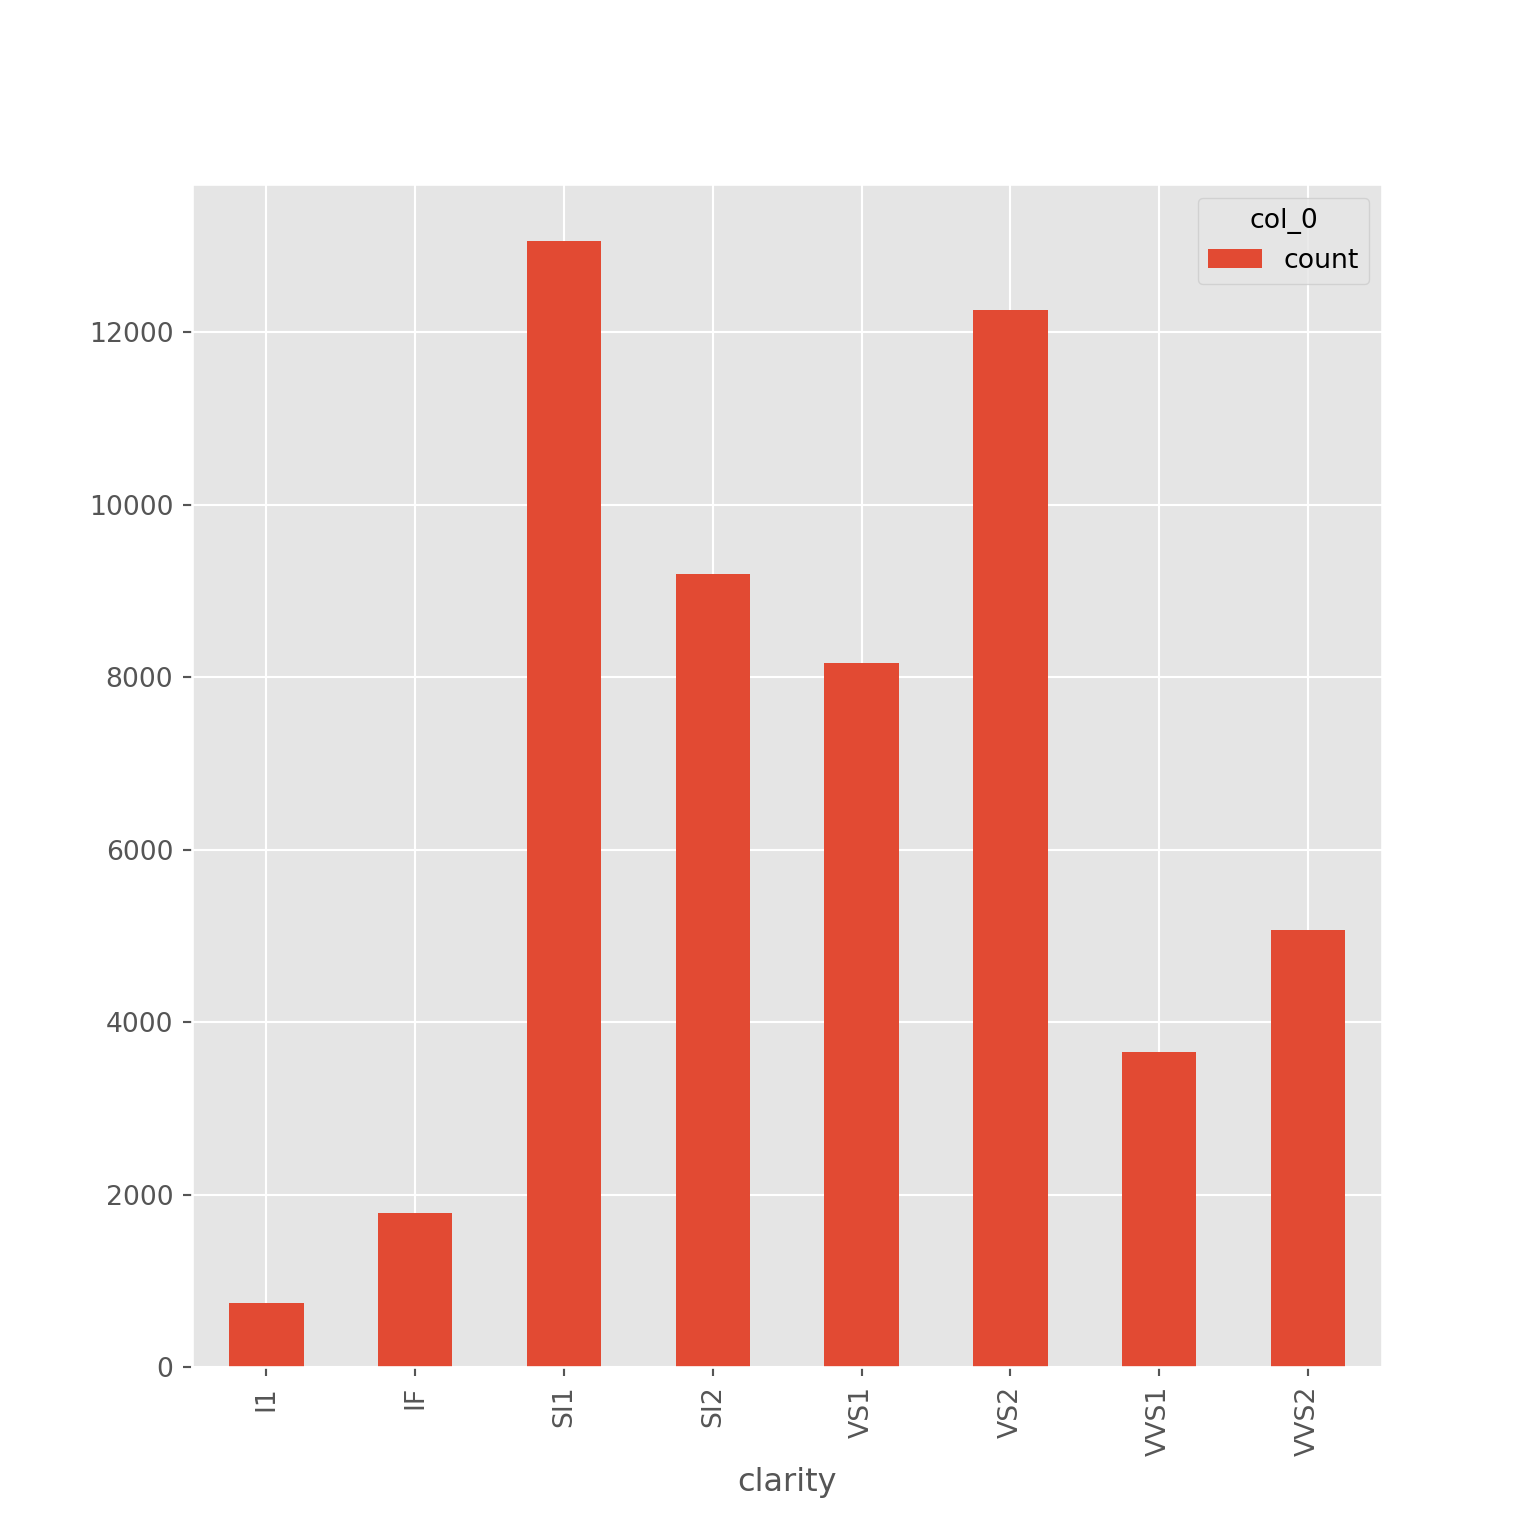
\includegraphics{SECCION-12_files/figure-latex/unnamed-chunk-8-1.pdf}

\hypertarget{anuxe1lisis-de-datos-ordinales-por-factor}{%
\section{ANÁLISIS DE DATOS ORDINALES POR
FACTOR}\label{anuxe1lisis-de-datos-ordinales-por-factor}}

Para calcular frecuencias acumuladas en una tabla multidimensional, hay
que aplicar a la tabla la funciopn cumsum mediante la funcion apply que
ya explicabamos para matrices. En este caso concreto, al sintaxis de la
instrucción sería

apply(tabla,MARGIN=\ldots,FUN=cumsum)

donde el valor de MARGIN ha de ser el de la dimension en la que queremos
acumular las frecuencias 1 si queremso hacerlo por filas 2 por si
queremos hacerlo por columans etc.

\hypertarget{ejemplo-4}{%
\subsection{EJEMPLO 4}\label{ejemplo-4}}

Supongamos que en el ejemplo anterior, el de las jirafas, estas
provienen de 4 zonas diferentes, a,B,C,D de manera que las 30 primeras
son de la zona A, las siguientes 25 son de la zona B, las 35 siguientes
de la zona C y las ultimas 10 de la zona D. Nos interesa estudiar la
distribución de las longitusdes según la zona.

Vamos a organizasr todos estos datos en un dataframe llamado jirafas.
Para q ue nos sea más fácil visualizar la información es conveniente que
las filas de las tablas de frecuencais correspondan a las zonas. Por lo
tanto, al definir el dataframe, entraremos como primera variable la de
la muestra de las zonas. Así conseguiremos que éstas aparezcan en las
filas al aplicarle la función table.

\begin{Shaded}
\begin{Highlighting}[]
\NormalTok{zonas}\OtherTok{=}\FunctionTok{rep}\NormalTok{(}\FunctionTok{c}\NormalTok{(}\StringTok{"A"}\NormalTok{,}\StringTok{"B"}\NormalTok{,}\StringTok{"C"}\NormalTok{,}\StringTok{"D"}\NormalTok{),}\FunctionTok{c}\NormalTok{(}\DecValTok{30}\NormalTok{,}\DecValTok{25}\NormalTok{,}\DecValTok{35}\NormalTok{,}\DecValTok{10}\NormalTok{))}
\NormalTok{jirafas}\OtherTok{=}\FunctionTok{data.frame}\NormalTok{(zonas,longitud)}
\NormalTok{jirafas}\SpecialCharTok{$}\NormalTok{zonas}\OtherTok{=}\FunctionTok{as.factor}\NormalTok{(jirafas}\SpecialCharTok{$}\NormalTok{zonas)}
\FunctionTok{str}\NormalTok{(jirafas)}
\end{Highlighting}
\end{Shaded}

\begin{verbatim}
'data.frame':   100 obs. of  2 variables:
 $ zonas   : Factor w/ 4 levels "A","B","C","D": 1 1 1 1 1 1 1 1 1 1 ...
 $ longitud: chr  "Largo" "Corto" "Muy largo" "Normal" ...
\end{verbatim}

\begin{Shaded}
\begin{Highlighting}[]
\FunctionTok{head}\NormalTok{(jirafas)}
\end{Highlighting}
\end{Shaded}

\begin{verbatim}
  zonas  longitud
1     A     Largo
2     A     Corto
3     A Muy largo
4     A    Normal
5     A Muy corto
6     A     Largo
\end{verbatim}

\hypertarget{para-calcular-la-tabla-de-frecuencacis-absolutas-acumuladas}{%
\subsubsection{PARA CALCULAR LA TABLA DE FRECUENCACIS ABSOLUTAS
ACUMULADAS}\label{para-calcular-la-tabla-de-frecuencacis-absolutas-acumuladas}}

Para calcular la tabla de frecuencias absolutas acumuladas de las
longitudes por zonas y como las zonas definen las filas de la tabla
anterior, debemos utilizar la funcion apply con MARGIN=1.

\begin{Shaded}
\begin{Highlighting}[]
\FunctionTok{apply}\NormalTok{(}\FunctionTok{table}\NormalTok{(jirafas), }\AttributeTok{MARGIN=}\DecValTok{1}\NormalTok{,}\AttributeTok{FUN=}\NormalTok{cumsum)}
\end{Highlighting}
\end{Shaded}

\begin{verbatim}
           zonas
longitud     A  B  C  D
  Corto      6  6  6  4
  Largo     12 11 14  5
  Muy corto 15 18 18  9
  Muy largo 20 23 25 10
  Normal    30 25 35 10
\end{verbatim}

\begin{Shaded}
\begin{Highlighting}[]
\FunctionTok{t}\NormalTok{(}\FunctionTok{apply}\NormalTok{(}\FunctionTok{table}\NormalTok{(jirafas), }\AttributeTok{MARGIN=}\DecValTok{1}\NormalTok{,}\AttributeTok{FUN=}\NormalTok{cumsum))}
\end{Highlighting}
\end{Shaded}

\begin{verbatim}
     longitud
zonas Corto Largo Muy corto Muy largo Normal
    A     6    12        15        20     30
    B     6    11        18        23     25
    C     6    14        18        25     35
    D     4     5         9        10     10
\end{verbatim}

Para calcular la tabla de frecuencias relativas acumuladas de las
longitudes del cuello po zonas. Para conseguirlo, y en una unica
instruccion, primero calculamos la tabla de frecuencias relativas por
filas, a continuación, con las funciones apply y cumsum las acumulamos y
finalmente transponemos el resultado.

\begin{Shaded}
\begin{Highlighting}[]
\FunctionTok{t}\NormalTok{(}\FunctionTok{apply}\NormalTok{(}\FunctionTok{prop.table}\NormalTok{(}\FunctionTok{table}\NormalTok{(jirafas),}\AttributeTok{margin=}\DecValTok{1}\NormalTok{),}\AttributeTok{MARGIN=}\DecValTok{1}\NormalTok{, }\AttributeTok{FUN=}\NormalTok{cumsum))}
\end{Highlighting}
\end{Shaded}

\begin{verbatim}
     longitud
zonas     Corto Largo Muy corto Muy largo Normal
    A 0.2000000  0.40 0.5000000 0.6666667      1
    B 0.2400000  0.44 0.7200000 0.9200000      1
    C 0.1714286  0.40 0.5142857 0.7142857      1
    D 0.4000000  0.50 0.9000000 1.0000000      1
\end{verbatim}

\hypertarget{diagrama-de-barras}{%
\subsubsection{DIAGRAMA DE BARRAS}\label{diagrama-de-barras}}

\begin{Shaded}
\begin{Highlighting}[]
\NormalTok{Diagrama}\OtherTok{=}\FunctionTok{apply}\NormalTok{(}\FunctionTok{prop.table}\NormalTok{(}\FunctionTok{table}\NormalTok{(jirafas),}\AttributeTok{margin =} \DecValTok{1}\NormalTok{),}\AttributeTok{MARGIN=}\DecValTok{1}\NormalTok{, }\AttributeTok{FUN=}\NormalTok{cumsum)}
\FunctionTok{barplot}\NormalTok{(Diagrama,}\AttributeTok{beside=}\ConstantTok{TRUE}\NormalTok{,}\AttributeTok{legend=}\ConstantTok{TRUE}\NormalTok{,}\AttributeTok{main=}\StringTok{"Diagrama de barras de frecuencias relativas acumuladas de longitudes por zonas"}\NormalTok{,}\AttributeTok{args.legend=}\FunctionTok{list}\NormalTok{(}\AttributeTok{x=}\StringTok{"topleft"}\NormalTok{,}\AttributeTok{cex=}\FloatTok{0.5}\NormalTok{),}\AttributeTok{col =} \FunctionTok{c}\NormalTok{(}\StringTok{"Red"}\NormalTok{,}\StringTok{"Green"}\NormalTok{,}\StringTok{"Blue"}\NormalTok{,}\StringTok{"Brown"}\NormalTok{,}\StringTok{"Pink"}\NormalTok{))}
\end{Highlighting}
\end{Shaded}

\includegraphics{SECCION-12_files/figure-latex/unnamed-chunk-12-1.pdf}

\hypertarget{ejemplo-5}{%
\subsection{EJEMPLO 5}\label{ejemplo-5}}

Consideremos el dataframe \textbf{datacrab} y arreglemos los datos

\begin{Shaded}
\begin{Highlighting}[]
\NormalTok{cangrejos}\OtherTok{=}\FunctionTok{read.table}\NormalTok{(}\StringTok{"r{-}basic{-}master/data/datacrab.txt"}\NormalTok{,}\AttributeTok{header =} \ConstantTok{TRUE}\NormalTok{)}
\NormalTok{cangrejos}\OtherTok{=}\NormalTok{cangrejos[,}\SpecialCharTok{{-}}\DecValTok{1}\NormalTok{]}\CommentTok{\#Omitimos la primera columna}
\FunctionTok{str}\NormalTok{(cangrejos)}
\end{Highlighting}
\end{Shaded}

\begin{verbatim}
## 'data.frame':    173 obs. of  5 variables:
##  $ color : int  3 4 2 4 4 3 2 4 3 4 ...
##  $ spine : int  3 3 1 3 3 3 1 2 1 3 ...
##  $ width : num  28.3 22.5 26 24.8 26 23.8 26.5 24.7 23.7 25.6 ...
##  $ satell: int  8 0 9 0 4 0 0 0 0 0 ...
##  $ weight: int  3050 1550 2300 2100 2600 2100 2350 1900 1950 2150 ...
\end{verbatim}

La variable width contiene la acnhura de cada cangrejo. Para comprobar
si es una variable ordinal podemos definir lo siguiente:

\begin{Shaded}
\begin{Highlighting}[]
\FunctionTok{table}\NormalTok{(cangrejos}\SpecialCharTok{$}\NormalTok{width)}
\end{Highlighting}
\end{Shaded}

\begin{verbatim}
  21   22 22.5 22.9   23 23.1 23.2 23.4 23.5 23.7 23.8 23.9   24 24.1 24.2 24.3 
   1    1    3    3    2    3    1    1    1    3    3    1    2    1    2    2 
24.5 24.7 24.8 24.9   25 25.1 25.2 25.3 25.4 25.5 25.6 25.7 25.8 25.9   26 26.1 
   7    5    1    3    6    2    2    1    3    3    2    6    7    1    6    2 
26.2 26.3 26.5 26.7 26.8   27 27.1 27.2 27.3 27.4 27.5 27.6 27.7 27.8 27.9   28 
   8    1    6    3    3    5    2    2    1    3    6    1    2    2    2    3 
28.2 28.3 28.4 28.5 28.7 28.9   29 29.3 29.5 29.7 29.8   30 30.2 30.3 30.5 31.7 
   4    3    2    4    2    1    6    2    1    1    1    3    1    1    1    1 
31.9 33.5 
   1    1 
\end{verbatim}

Como podemos ver no es una variable ordinal, apra convertirla en
variable ordinal utilizando escalas hacemos lo siguiente:

La manera msa sencilla de dividirlo por segmentos es utilizar la funcion
cut, que estudiaremos en detalle en lecciones posteriores. Por ahora,
basta con saber que la instrucción dividirá el vector numérico
crabs\$width en intervalos de extremos los puntos específicados en el
argumento breaks. El parámetro right=FALSE sirve para indicar que los
puntos de corte pertenecen al intervalo de su derecha e Inf indica
infinito. RIGHT=FALSE dice que es intervalo abierto es decir, si tenemos
el intervalo 24-25 el 25 no esta incluido dentro del intervalo.

\begin{Shaded}
\begin{Highlighting}[]
\NormalTok{intervalos}\OtherTok{=}\FunctionTok{cut}\NormalTok{(cangrejos}\SpecialCharTok{$}\NormalTok{width,}\AttributeTok{breaks =} \FunctionTok{c}\NormalTok{(}\DecValTok{21}\NormalTok{,}\DecValTok{25}\NormalTok{,}\DecValTok{29}\NormalTok{,}\DecValTok{33}\NormalTok{,}\ConstantTok{Inf}\NormalTok{),}\AttributeTok{right =} \ConstantTok{FALSE}\NormalTok{,}\AttributeTok{labels =} \FunctionTok{c}\NormalTok{(}\StringTok{"21{-}25"}\NormalTok{,}\StringTok{"25{-}29"}\NormalTok{,}\StringTok{"29{-}33"}\NormalTok{,}\StringTok{"33{-}..."}\NormalTok{))}
\end{Highlighting}
\end{Shaded}

Para ordenar dichos rangos hacemos lo siguiente:

\begin{Shaded}
\begin{Highlighting}[]
\NormalTok{cangrejos}\SpecialCharTok{$}\NormalTok{width.rank}\OtherTok{=}\FunctionTok{ordered}\NormalTok{(intervalos)}
\FunctionTok{str}\NormalTok{(cangrejos)}
\end{Highlighting}
\end{Shaded}

\begin{verbatim}
'data.frame':   173 obs. of  6 variables:
 $ color     : int  3 4 2 4 4 3 2 4 3 4 ...
 $ spine     : int  3 3 1 3 3 3 1 2 1 3 ...
 $ width     : num  28.3 22.5 26 24.8 26 23.8 26.5 24.7 23.7 25.6 ...
 $ satell    : int  8 0 9 0 4 0 0 0 0 0 ...
 $ weight    : int  3050 1550 2300 2100 2600 2100 2350 1900 1950 2150 ...
 $ width.rank: Ord.factor w/ 4 levels "21-25"<"25-29"<..: 2 1 2 1 2 1 2 1 1 2 ...
\end{verbatim}

Si nos interesa estudiar la distribución de las anchuras de los
cangrejos segun el numero de colores. Por lo tanto, vamos a calcular las
tablas bidimensionales de frecuencais relativas y relativas acumuladas
de los intervalos de las anchuras en cada nivel de color y las
representaremos por medio de diagramas de barras.

La tabla de frecuencias de los pares se puede obtener aplicando table al
dataframe formado por la primera y ultima columnas.

\begin{Shaded}
\begin{Highlighting}[]
\NormalTok{Tabla}\OtherTok{=}\FunctionTok{table}\NormalTok{(cangrejos[,}\FunctionTok{c}\NormalTok{(}\DecValTok{1}\NormalTok{,}\DecValTok{6}\NormalTok{)])}
\NormalTok{Tabla}
\end{Highlighting}
\end{Shaded}

\begin{verbatim}
     width.rank
color 21-25 25-29 29-33 33-...
    2     1     9     2      0
    3    19    62    13      1
    4    17    24     3      0
    5     9    12     1      0
\end{verbatim}

Para obtener la tabla de frecuencias relativas se usa la siguiente
instruccion:

\begin{Shaded}
\begin{Highlighting}[]
\NormalTok{frecRel}\OtherTok{=}\FunctionTok{round}\NormalTok{(}\FunctionTok{prop.table}\NormalTok{(Tabla,}\AttributeTok{margin =} \DecValTok{1}\NormalTok{),}\DecValTok{3}\NormalTok{)}
\NormalTok{frecRel}
\end{Highlighting}
\end{Shaded}

\begin{verbatim}
     width.rank
color 21-25 25-29 29-33 33-...
    2 0.083 0.750 0.167  0.000
    3 0.200 0.653 0.137  0.011
    4 0.386 0.545 0.068  0.000
    5 0.409 0.545 0.045  0.000
\end{verbatim}

Para obtener la tabla de frecuencias relativas acumulada se utiliza la
siguiente instrucción:

\begin{Shaded}
\begin{Highlighting}[]
\NormalTok{frecRelAcum}\OtherTok{=}\FunctionTok{round}\NormalTok{(}\FunctionTok{apply}\NormalTok{(}\FunctionTok{prop.table}\NormalTok{(Tabla,}\AttributeTok{margin=}\DecValTok{1}\NormalTok{), }\AttributeTok{MARGIN=}\DecValTok{1}\NormalTok{, }\AttributeTok{FUN=}\NormalTok{cumsum),}\DecValTok{3}\NormalTok{)}
\FunctionTok{t}\NormalTok{(frecRelAcum)}
\end{Highlighting}
\end{Shaded}

\begin{verbatim}
     width.rank
color 21-25 25-29 29-33 33-...
    2 0.083 0.833 1.000      1
    3 0.200 0.853 0.989      1
    4 0.386 0.932 1.000      1
    5 0.409 0.955 1.000      1
\end{verbatim}

Graficando en diagramas de barras tenemos lo siguiente:

\begin{Shaded}
\begin{Highlighting}[]
\NormalTok{azul}\OtherTok{=}\FunctionTok{c}\NormalTok{(}\StringTok{"cyan"}\NormalTok{,}\StringTok{"cyan4"}\NormalTok{,}\StringTok{"cyan1"}\NormalTok{,}\StringTok{"cyan3"}\NormalTok{)}
\FunctionTok{barplot}\NormalTok{(}\FunctionTok{t}\NormalTok{(frecRel),}
        \AttributeTok{beside =} \ConstantTok{TRUE}\NormalTok{,}
        \AttributeTok{legend=}\ConstantTok{TRUE}\NormalTok{,}
        \AttributeTok{ylim=}\FunctionTok{c}\NormalTok{(}\DecValTok{0}\NormalTok{,}\DecValTok{1}\NormalTok{),}
        \AttributeTok{col=}\NormalTok{azul,}
        \AttributeTok{main=}\StringTok{"Diagrama de barras de frecuencais relativas"}\NormalTok{,}
        \AttributeTok{args.legend=}\FunctionTok{list}\NormalTok{(}\AttributeTok{x=}\StringTok{"topright"}\NormalTok{,}\AttributeTok{cex=}\FloatTok{0.55}\NormalTok{))}
\end{Highlighting}
\end{Shaded}

\includegraphics{SECCION-12_files/figure-latex/unnamed-chunk-20-1.pdf}

Graficando el grafico de frecuencias relativas acumuladas.

\begin{Shaded}
\begin{Highlighting}[]
\FunctionTok{barplot}\NormalTok{(frecRelAcum,}
        \AttributeTok{beside =} \ConstantTok{TRUE}\NormalTok{,}
        \AttributeTok{legend=}\ConstantTok{TRUE}\NormalTok{,}
        \AttributeTok{col=}\NormalTok{azul,}
        \AttributeTok{main=}\StringTok{"Diagrama de barras de frecuencias acumuladas"}\NormalTok{,}
        \AttributeTok{args.legend=}\FunctionTok{list}\NormalTok{(}\AttributeTok{x=}\StringTok{"topleft"}\NormalTok{,}\AttributeTok{cex=}\FloatTok{0.55}\NormalTok{)}
\NormalTok{        )}
\end{Highlighting}
\end{Shaded}

\includegraphics{SECCION-12_files/figure-latex/unnamed-chunk-21-1.pdf}

\end{document}
